\subsubsection{二つの点を参照して次の点を選択する場合(case 4, case 5)}

次に、過去の二つの選択された点を参照して、その2点から近い位置にあるてんを次に選ばれる点の候補とする場合を考えることにする。このとき、2点からの近さの指標は、うまくこちらで決めてやる必要がある。近さの指標となる一つの例として、二つの点を焦点とした楕円を考えることができる。すなわち2つの点からの距離の和が等しい点はすべて同じ距離にあると見なすような近さが考えられる。したがって2点$(y, z)$からの点$x$の近さの指標$D(x, (y, z))$は、通常の$a$次元ユークリッド次元を$d(x,y)$と表すと、
$$D(x, (y, z)) = d(x,y) + d(x, z)$$
のように書けることになる。また、この考えが役に立つのは、それぞれの距離を足すときに適当な正の係数を掛けることによって、2つの点のどちらへの近さを優先するのかという条件を付け加えることができる点である。すなわち、正の定数$\alpha$ ,$\beta$を用いて、
$$D(x, (y, z)) = \alpha d(x,y) + \beta d(x, z)$$
のようにも書くことができる。参照する点をさらに増やしたい場合にも、それらの点との間の距離に係数を掛けて足せばよいので、いくらでも参照点を増やすことは可能である:
$$D(x_{k+1}, (x_{1}, x_{2}, \cdots , x_{k})) = \sum_{i=1}^{k}w_{i}d(x_{k+1}, x_{i})\ \ (w_{i} > 0)$$
また、別の近さの指標として、ベクトル$\vec{Y} = y-x$, $\vec{Z} = z-x$として
$$D(x, (y,z)) = |t\vec{Y} + (1-t)\vec{Z}|\ \ (0 \le t \le 1)$$
とする方法もある。このとき、右辺の括弧の内部が表すベクトルは、点$y$,$z$を結んだ線分$YZ$を$(1-t):1$に内分する点のベクトルを示しており、$D$はその点から$x$までのユークリッド距離を表すことになる。

シミュレーションでは、はじめに挙げた近さの指標を用いて選択権の順番を決定することにする、図\ref{fig:f11}と図\ref{fig:f12}は、それぞれ$x_{0}$の点と一つ前の点を参照にして点を選択する場合と、二つ前までの点を参照にして点を選択する場合のシミュレーションを行ったときに得られた結果の例である。

\begin{figure}[H]
    \begin{center}
        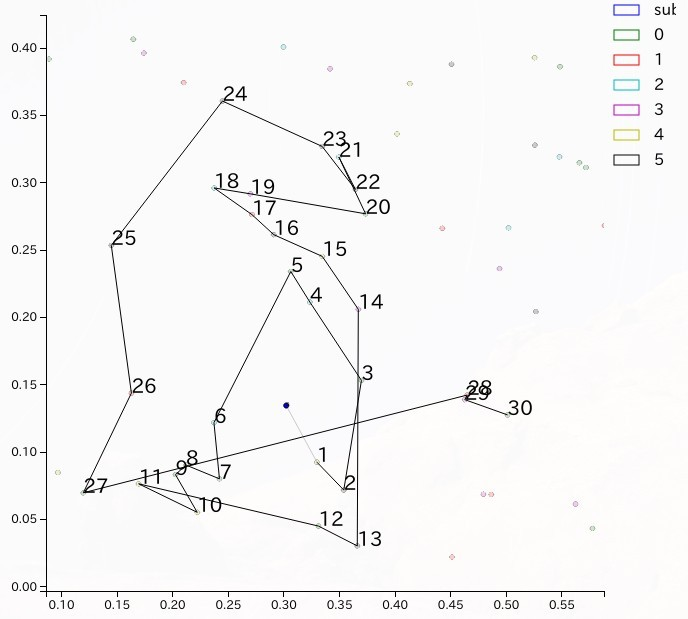
\includegraphics[width=10cm]{../simple3/case_4.jpg}
        \caption{$x_{0}$と一つ前の点を参照にして次の点を選んだ場合(case 4)のシミュレーション結果の一例}
        \label{fig:f11}
    \end{center}
\end{figure}
\begin{figure}[H]
    \begin{center}
        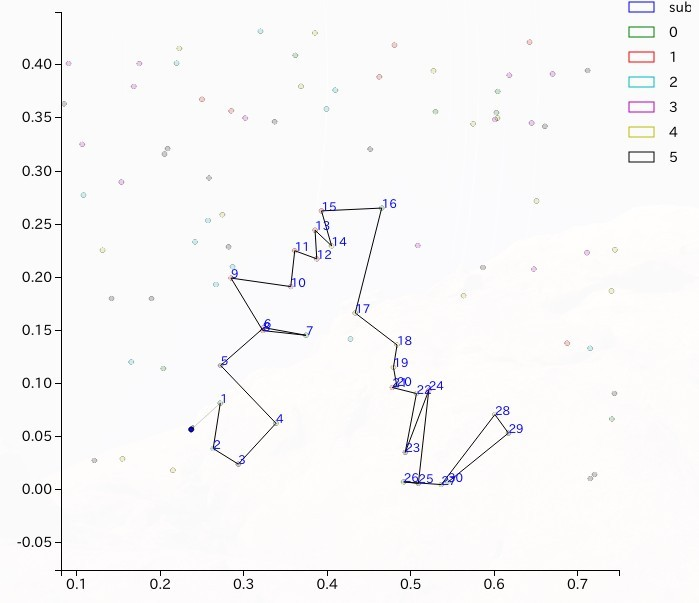
\includegraphics[width=10cm]{../simple3/case_5.jpg}
        \caption{二つ前までの点を参照にして次の点を選んだ場合(case 5)のシミュレーション結果の一例}
        \label{fig:f12}
    \end{center}
\end{figure}

\subsubsection{結果と考察}

システムサイズと系の特徴量の間の関係を知りたいので、$X_{i}$の数$N$を変えたときの軌跡の性質を調べた。他の条件を揃えたまま$N$のみを変化させたとき、各ステップの平均移動距離を計算し、プロットしたものを図\ref{fig:f13}に示す(試行は100回行った)。このグラフから分かるように、$N$が増加するほど1ステップあたりの平均移動距離は小さくなっていることが分かる。また、両軸を対数表示にした上で直線でフィッティングしたものを図\ref{fig:f14}に示すが、平均ステップ間距離は$N$に対してベキ的に減少しており、その傾きはおよそ-0.5であることが分かる。これは$N$の増大によって、各点の間の平均距離$r$自体が$N$に対して$1/2$乗ほどで減少していく効果がそのまま現れたものであると見ることができる。
\begin{figure}[H]
    \begin{center}
        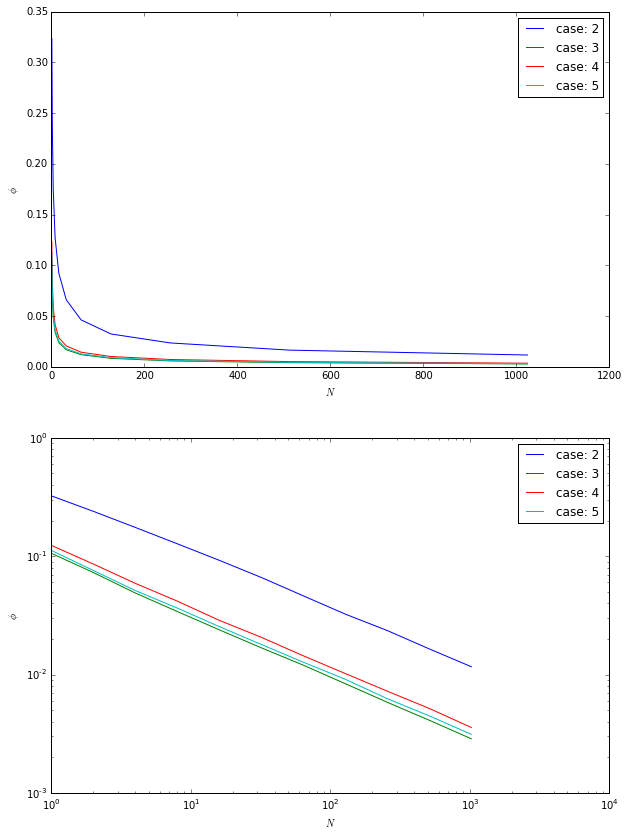
\includegraphics[width=12.5cm]{../img/simple3_N_2.png}
        \caption{$N$を変化させたときのステップ間の平均移動距離}
        \label{fig:f13}
    \end{center}
\end{figure}
\begin{figure}[H]
    \begin{center}
        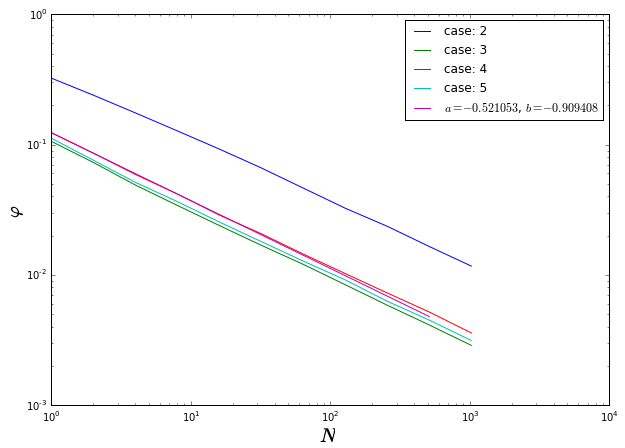
\includegraphics[width=12.5cm]{../img/simple3_N_2_fit.png}
        \caption{図\ref{fig:f13}の両対数グラフを直線でフィッティングしたもの}
        \label{fig:f14}
    \end{center}
\end{figure}
